\documentclass[8pt]{beamer}
\usefonttheme[onlymath]{serif}


\setbeamertemplate{frametitle}{%
  \vskip1ex
  \usebeamerfont{frametitle}%
  \insertsubsectionhead\par        %  ← 원하는 대로 변경 가능
  \vskip1ex
  \hrule                             % 밑줄(선택)
}

% 테마 선택 (선택 사항)
% \usetheme{Madrid} % 기본 테마, 다른 테마 사용 가능
% \font{serif}
\usepackage{amsfonts}
\usepackage{amssymb}
\usepackage[T1]{fontenc} % To use combination of textbf, textit
\usepackage[dvipsnames]{xcolor}   % can use more variant colors

\usepackage[
  backend=biber,
  style=authoryear,   % or numeric
  citestyle=authoryear
]{biblatex}
\addbibresource{../../references.bib}

% \setcounter{MaxMatrixCols}{20}

% (필요한 패키지들)
% \usepackage{amsthm}
\setbeamertemplate{theorems}[numbered]  % 정리, 정의 등에 번호를 달아줌

% \theoremstyle{plain} % insert bellow all blocks you want in italic
% \newtheorem{theorem}{Theorem}[section] % to number according to section
% 
% \theoremstyle{definition} % insert bellow all blocks you want in normal text
% \newtheorem{definition}{Definition}[section] % to number according to section
% \newtheorem*{idea}{Proof idea} % no numbered block

\newtheorem{proposition}[theorem]{Proposition}

\usepackage{tcolorbox}

% 필요할 경우 패키지 추가
\usepackage{graphicx} % 이미지 삽입을 위한 패키지
\usepackage{amsmath}   % 수식 사용
\usepackage{hyperref}  % 하이퍼링크 추가
\usepackage{cleveref}
\usepackage{multicol}  % 여러 열 나누기
\usepackage{ulem} % 취소선 및줄 나누기



\newcommand{\mrm}[1]{\mathrm{#1}}
\newcommand{\mbb}[1]{\mathbb{#1}}
\newcommand{\mb}[1]{\mathbf{#1}}
\newcommand{\mc}[1]{\mathcal{#1}}
\newcommand{\tb}[1]{\textbf{#1}}
\newcommand{\ti}[1]{\textit{#1}}
\newcommand{\mypois}[1]{\operatorname{Pois}(#1)}

\newcommand{\myber}[1]{\operatorname{Bern}\!\left(#1\right)}
\newcommand{\mybin}[2]{\operatorname{Bin}\!\left(#1,#2\right)}
\newcommand{\mytoinf}[1]{#1 \rightarrow \infty}
\newcommand{\myexp}[1]{\exp{\left(#1\right)}}
\newcommand{\myunif}[2]{\operatorname{Unif}\!\left(#1, #2\right)}
\newcommand{\mygeom}[1]{\operatorname{Geom}\!\left(#1\right)}
\newcommand{\myexpo}[1]{\operatorname{Expo}\!\left(#1\right)}
\newcommand{\abs}[1]{\left\lvert #1 \right\rvert}
\newcommand{\expec}[1]{\operatorname{E}\left[ #1 \right]}
\newcommand{\myvar}[1]{\operatorname{Var}\left[#1\right]}
\newcommand{\myskew}[1]{\operatorname{Skew}\!\left[#1\right]}
\newcommand{\mykurt}[1]{\operatorname{Kurt}\!\left[#1\right]}
\newcommand{\mywei}[2]{\operatorname{Wei}\!\left(#1, #2\right)}
\newcommand{\Span}[1]{\operatorname{Span}\!\left(#1\right)}
\newcommand{\softmax}[2]{\operatorname{softmax}_{#1}\!\left(#2\right)}

% 발표 제목, 저자, 날짜 설정
\title{Dueling DQN}
\author{Gwanwoo Choi}
% \date{}

\begin{document}
% 표지 슬라이드
\begin{frame}
    \titlepage
\end{frame}

\subsection{Algorithm explained}

% \begin{frame}
%     \frametitle{Table of Contents}
%     \tableofcontents[currentsubsection]
% \end{frame}

\begin{frame}{a}
    Dueling DQN suggests brand new structure for DQN based training.
    \begin{itemize}
        \item Explicitly separate 'State-Value' and 'Action-Value'
        \item In Dueling DQN, neural network produces $V(s)$ and $A(s,a)$ instead of $Q(s,a)$
        \item Note that in reinforcement learning, $Q(s,a)$ is represented by $V(s) + A(s,a)$
    \end{itemize}

    \begin{figure}
        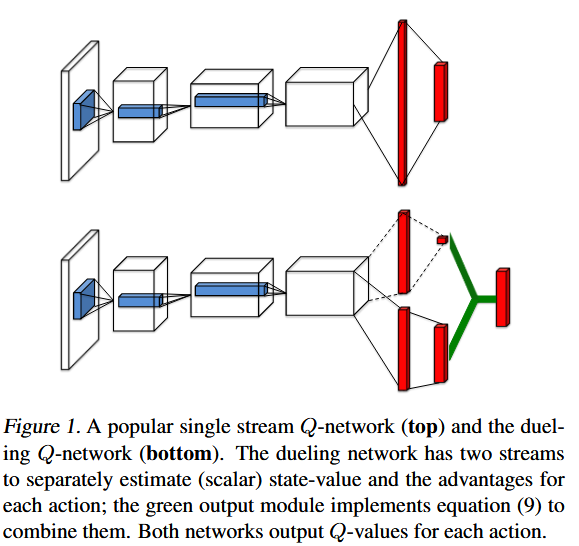
\includegraphics[width=0.5\textwidth]{DuelingDQNStructure.png}
    \end{figure}
    Although model structure is different, we can utilize same training framework such as DQN or Double DQN.
\end{frame}

\begin{frame}{a}
    Let's say process obtaining $Q(s,a)$ as $Q(s,a)= V(s) + A(s,a)$ as Naive Dueling DQN.

    There is problem in just adopting original DQN or Double DQN training method on Naive Dueling DQN framework.

    Q-learning Loss funtion in DQN is 
    \[
        L_\theta =  \left(r(s,a) + \gamma \max_{a^\prime} Q_{\bar{\theta}}(s^\prime, a^\prime) - Q_\theta(s,a) \right)^2
    \]
    But in Naive Dueling DQN, $Q_{\theta, \alpha, \beta}(s,a) = V_{\theta, \alpha}(s) + A_{\theta,\beta} (s,a)$ and Q-learning Loss function becomes
    \[
        L_{\alpha, \beta} = \left( r(s,a) + V_{\bar{\alpha}}(s^\prime) + \gamma \max_{a^\prime} A_{\bar{\beta}}(s^\prime, a^\prime) - V_\alpha (s) - A_\beta (s,a)  \right)^2
    \]
    \begin{itemize}
        \item $\theta$ represents parameters preceded both $V$ and $A$ network branch
        \item $\alpha$ represents independent network branch of $V$ and $\beta$ represents independent network branch of $A$
    \end{itemize}

\end{frame}

\begin{frame}{a}
    Note that for all constant $C$, under loss function is same loss function with Naive Dueling DQN
    \[
        L_{\alpha, \beta} = \left( r(s,a) + V_{\bar{\alpha}}(s^\prime) + \gamma \max_{a^\prime} A_{\bar{\beta}}(s^\prime, a^\prime) - (V_\alpha (s)+C) - (A_\beta (s,a)-C)  \right)^2
    \]

    This leads unstability of training.

    How can we fix it? In dueling DQN paper, three methods is presented
    \begin{enumerate}
        \item $Q_{\theta, \alpha, \beta}(s,a) = V_{\theta, \alpha} (s) + (A_{\theta, \beta}(s,a) - \max_{a}A_{\theta, \beta}(s,a))$
        \item $Q_{\theta, \alpha, \beta}(s,a) = V_{\theta, \alpha}(s) + (A_{\theta, \beta}(s,a) - \sum_{a \in \mc{A}} A_{\theta, \beta}(s,a)/\abs{\mc{A}})$
        \item $Q_{\theta, \alpha, \beta}(s,a) = V_{\theta, \alpha}(s) + (A_{\theta, \beta} - \softmax{a}{A_{\theta, \beta} (s,a)}) $
    \end{enumerate}

    Paper said that $2 > 1$ (2 shows better performance than 1) and $3 \simeq 2$ (3 shows similar performance with 2). In paper all experiments utilize equation $2$.
\end{frame}

\subsection{Experiment setting}

% \begin{frame}{a}
%     \tableofcontents[currentsubsection]
% \end{frame}

\begin{frame}{.}
    My Experiment setting is Below. 
    \begin{itemize}
        \item Training is based on DQN algorithm and detailed explanation is in [\cite{mnih2015human}]
        \item Buffer size: $0.1M$ (\cite{mnih2015human} algorithm uses $1M$)
        \item behavior policy : $\epsilon$-greedy with annealing $\epsilon : 1 \rightarrow 0.1$ in first $1M$ timestep
        \item target policy: $\epsilon$-greedy with $\epsilon: 0.5$
        \item Total timestep : $2.5M$ (\cite{mnih2015human} algorithm uses $50M$)
        \item Same CNN structure except $V$ network and $A$ network
        \item Target Network update frequency: $500$ (\cite{mnih2015human} is $10000$)
        \item Minibatch size : $256$ (\cite{mnih2015human} is $32$)
    \end{itemize}
\end{frame}

\begin{frame}{.}
    \begin{columns}
        \begin{column}{0.45\textwidth}
            Right figure is Network architecture for Atari games (especially breakout)
            \begin{itemize}
                \item CNN network architecrue preceded MLP networks is the same structure with original DQN
                \item After CNN there exists two branch for calculating $Q$ and $V$
            \end{itemize}
        \end{column}
        \begin{column}{0.55\textwidth}
            \begin{figure}
                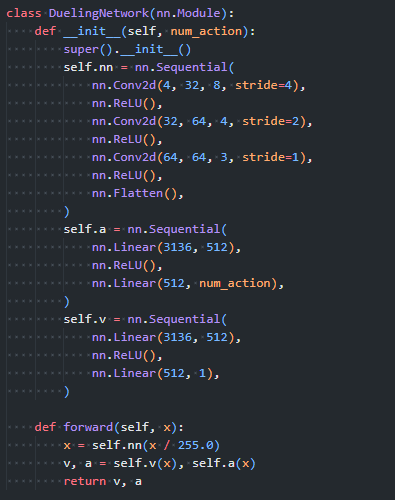
\includegraphics[width=0.95\textwidth]{DuelingDQNNetwork.png}
            \end{figure}
        \end{column}
    \end{columns}
\end{frame}

\begin{frame}{.}
    \begin{figure}
        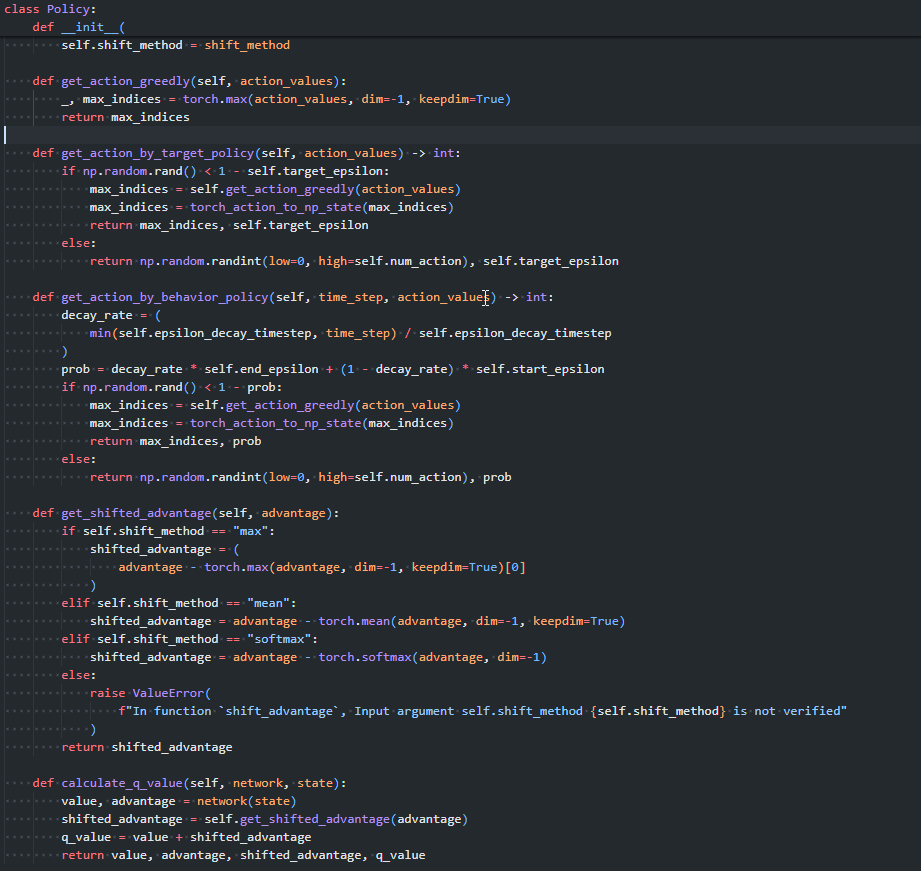
\includegraphics[width=0.8\textwidth]{DuelingDQNPolicyCode.png}
    \end{figure}
\end{frame}

\begin{frame}{.}
    In above code snippet, in `get\_shifted\_advantage` function, $Q$ is calculated based on $V$ and $A$.

    I experiment with method `mean`, which calculating $Q$ by
    $Q_{\theta, \alpha, \beta}(s,a) = V_{\theta, \alpha}(s) + (A_{\theta, \beta}(s,a) - \sum_{a \in \mc{A}} A_{\theta, \beta}(s,a)/\abs{\mc{A}})$

    And other parts of code are almost same with original DQN. For example, obtaining loss function process is same.

    \begin{figure}
        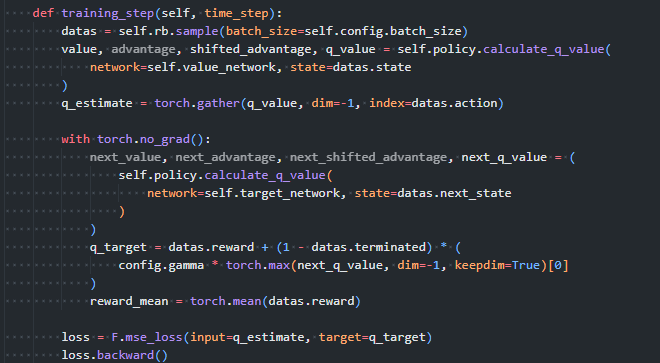
\includegraphics[width=0.85\textwidth]{DuelingDQNLoss.png}
    \end{figure}
\end{frame}

\subsection{Experiment result}

\begin{frame}{.}
    I found that there exists performance drop after about $1M$ timesteps.
    \begin{figure}
        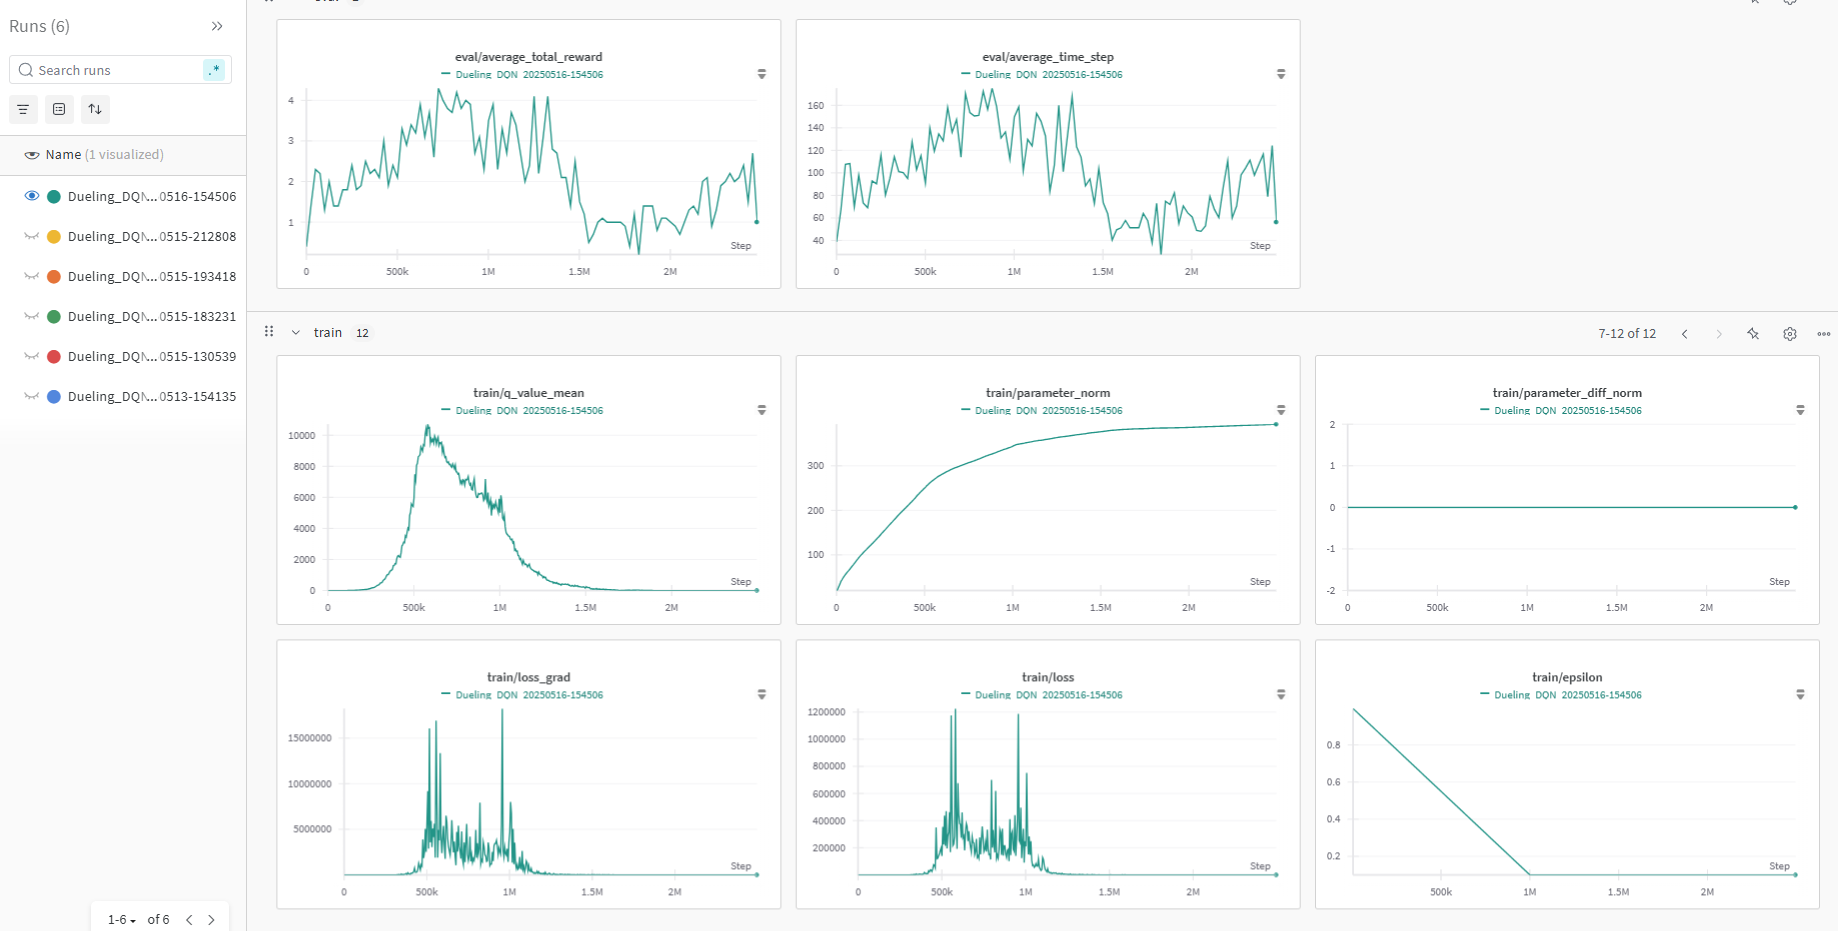
\includegraphics[width=0.9\textwidth]{DuelingDQNExp1_1.png}
    \end{figure}
\end{frame}

\begin{frame}{.}
    More stuff to experiment (to do)
    \begin{itemize}
        \item Increase total timestep (up to $10M$ timesteps), because in \cite{mnih2015human}, total timestep is 50M
        \item Since replay buffer size is $0.1M$, which is much smaller than \cite{mnih2015human} ($1M$), it seems that increasing $\epsilon$ ($0.1 \rightarrow 0.2$) of behavior policy or increasing annealing timestep ($1M \rightarrow 5M$) can show better performance
        \item Increase target network frequency $500 \rightarrow 10000$
    \end{itemize}
\end{frame}

\subsection{References}
\begin{frame}[allowframebreaks]{References}
  \printbibliography
\end{frame}

\end{document}